

\documentclass[useAMS,usenatbib]{mn2e}

% The usenatbib command allows the use of Patrick Daly's natbib.sty for
% cross-referencing.
%
% If you wish to typeset the paper in Times font (if you do not have the
% PostScript Type 1 Computer Modern fonts you will need to do this to get
% smoother fonts in a PDF file) then uncomment the next line
% \usepackage{Times}

%%%%% AUTHORS - PLACE YOUR OWN MACROS HERE %%%%%
%  These Macros are taken from the AAS TeX macro package version 4.0.
%  Include this file in your LaTeX source only if you are not using
%  the AAS TeX macro package and need to resolve the macro definitions
%  in the BibTeX entries returned by the ADS abstract service.
%
%  If you plan not to use this file to resolve the journal macros
%  rather than the whole AAS TeX macro package, you should save the
%  file as ``aas_macros.sty'' and then include it in your paper by
%  using a construct such as:
%\documentstyle[11pt,aas_macros]{article}
%
%  For more information on the AASTeX macro package, please see the URL
%http://www.aas.org/publications/aastex.html
%  For more information about ADS abstract server, please see the URL
%http://adswww.harvard.edu/ads_abstracts.html
%

% Abbreviations for journals.  The object here is to provide authors
% with convenient shorthands for the most ``popular'' (often-cited)
% journals; the author can use these markup tags without being concerned
% about the exact form of the journal abbreviation, or its formatting.
% It is up to the keeper of the macros to make sure the macros expand
% to the proper text.  If macro package writers agree to all use the
% same TeX command name, authors only have to remember one thing, and
% the style file will take care of editorial preferences.  This also
% applies when a single journal decides to revamp its abbreviating
% scheme, as happened with the ApJ (Abt 1991).

\let\jnlstyle=\rm
\def\refjnl#1{{\jnlstyle#1}}

\def\aj{\refjnl{AJ}}                   % Astronomical Journal
\def\araa{\refjnl{ARA\&A}}             % Annual Review of Astron and Astrophys
\def\apj{\refjnl{ApJ}}                 % Astrophysical Journal
\def\apjl{\refjnl{ApJ}}                % Astrophysical Journal, Letters
\def\apjs{\refjnl{ApJS}}               % Astrophysical Journal, Supplement
\def\ao{\refjnl{Appl.~Opt.}}           % Applied Optics
\def\apss{\refjnl{Ap\&SS}}             % Astrophysics and Space Science
\def\aap{\refjnl{A\&A}}                % Astronomy and Astrophysics
\def\aapr{\refjnl{A\&A~Rev.}}          % Astronomy and Astrophysics Reviews
\def\aaps{\refjnl{A\&AS}}              % Astronomy and Astrophysics, Supplement
\def\azh{\refjnl{AZh}}                 % Astronomicheskii Zhurnal
\def\baas{\refjnl{BAAS}}               % Bulletin of the AAS
\def\jrasc{\refjnl{JRASC}}             % Journal of the RAS of Canada
\def\memras{\refjnl{MmRAS}}            % Memoirs of the RAS
\def\mnras{\refjnl{MNRAS}}             % Monthly Notices of the RAS
\def\pra{\refjnl{Phys.~Rev.~A}}        % Physical Review A: General Physics
\def\prb{\refjnl{Phys.~Rev.~B}}        % Physical Review B: Solid State
\def\prc{\refjnl{Phys.~Rev.~C}}        % Physical Review C
\def\prd{\refjnl{Phys.~Rev.~D}}        % Physical Review D
\def\pre{\refjnl{Phys.~Rev.~E}}        % Physical Review E
\def\prl{\refjnl{Phys.~Rev.~Lett.}}    % Physical Review Letters
\def\pasp{\refjnl{PASP}}               % Publications of the ASP
\def\pasj{\refjnl{PASJ}}               % Publications of the ASJ
\def\qjras{\refjnl{QJRAS}}             % Quarterly Journal of the RAS
\def\skytel{\refjnl{S\&T}}             % Sky and Telescope
\def\solphys{\refjnl{Sol.~Phys.}}      % Solar Physics
\def\sovast{\refjnl{Soviet~Ast.}}      % Soviet Astronomy
\def\ssr{\refjnl{Space~Sci.~Rev.}}     % Space Science Reviews
\def\zap{\refjnl{ZAp}}                 % Zeitschrift fuer Astrophysik
\def\nat{\refjnl{Nature}}              % Nature
\def\iaucirc{\refjnl{IAU~Circ.}}       % IAU Cirulars
\def\aplett{\refjnl{Astrophys.~Lett.}} % Astrophysics Letters
\def\apspr{\refjnl{Astrophys.~Space~Phys.~Res.}}
                % Astrophysics Space Physics Research
\def\bain{\refjnl{Bull.~Astron.~Inst.~Netherlands}} 
                % Bulletin Astronomical Institute of the Netherlands
\def\fcp{\refjnl{Fund.~Cosmic~Phys.}}  % Fundamental Cosmic Physics
\def\gca{\refjnl{Geochim.~Cosmochim.~Acta}}   % Geochimica Cosmochimica Acta
\def\grl{\refjnl{Geophys.~Res.~Lett.}} % Geophysics Research Letters
\def\jcp{\refjnl{J.~Chem.~Phys.}}      % Journal of Chemical Physics
\def\jgr{\refjnl{J.~Geophys.~Res.}}    % Journal of Geophysics Research
\def\jqsrt{\refjnl{J.~Quant.~Spec.~Radiat.~Transf.}}
                % Journal of Quantitiative Spectroscopy and Radiative Transfer
\def\memsai{\refjnl{Mem.~Soc.~Astron.~Italiana}}
                % Mem. Societa Astronomica Italiana
\def\nphysa{\refjnl{Nucl.~Phys.~A}}   % Nuclear Physics A
\def\physrep{\refjnl{Phys.~Rep.}}   % Physics Reports
\def\physscr{\refjnl{Phys.~Scr}}   % Physica Scripta
\def\planss{\refjnl{Planet.~Space~Sci.}}   % Planetary Space Science
\def\procspie{\refjnl{Proc.~SPIE}}   % Proceedings of the SPIE

\let\astap=\aap
\let\apjlett=\apjl
\let\apjsupp=\apjs
\let\applopt=\ao


\input{psfig.sty}
\usepackage{graphicx}
\usepackage{epsfig}
\usepackage{amssymb}
\usepackage{amsmath}
\usepackage{amsfonts}
\usepackage{txfonts}

\title[{\small}  High Performance P$^{3}$M N-body code: CUBEP3M]{{\small} High Performance P$^{3}$M N-body code: CUBEP3M: }
\author[Joachim Harnois-D\'{e}raps, Ue-Li Pen, Ilian T. Iliev, Hugh Merz, JD Emberson, Vincent Desjacques]{Joachim Harnois-D\'{e}raps$^{1,2}$ 
\thanks{E-mail: jharno@cita.utoronto.ca},  Ue-Li Pen$^{1}$ \thanks{E-mail: pen@cita.utoronto.ca}, 
Ilian T. Iliev$^{3}$ \thanks{E-mail: i.t.iliev@sussex.ac.uk}, Hugh Merz$^{4}$ \thanks{E-mail: merz@sharcnet.ca}, \newauthor
JD Emberson$^{1,5}$ \thanks{E-mail: emberson@astro.utoronto.ca} and Vincent Desjacques$^{6,7}$ \thanks{E-mail:vincent.desjacques@unige.ch}\\
%\footnotemark[1]\thanks{This file has been amended to
%highlight the proper use of \LaTeXe\ code with the class file.
%These changes are for illustrative purposes and do not reflect the
%original paper by A. V. Raveendran.}\\
$^{1}$Canadian Institute for Theoretical Astrophysics, University of
Toronto, M5S 3H8, Ontario, Canada\\
$^{2}$Department of Physics, University of Toronto, M5S 1A7, Ontario,  Canada\\
$^{3}$Astronomy Centre, Department of Physics and Astronomy, Pevensey II Building, University of Sussex, BN1 9QH, Brighton, United Kingdom\\
$^{4}$Department of Mathematics and Computer Science, Laurentian University, P3E 2C6, Ontario, Canada\\
$^{5}$Department of Astronomy and Astrophysics, University of Toronto, M5S 3H4, Ontario, Canada\\
$^{6}$Institute for Theoretical Physics, University of Z\"{u}rich, Z\"{u}rich, CH 8057, Switzerland\\
$^{7}$Universit\'{e} de Gen\`{e}ve and Center for Astroparticle Physics, 24 Quai Ernest Ansermet, 1211 Gen\`{e}ve 4, Switzerland}

\begin{document}

%\date{Accepted 1988 December 15. Received 1988 December 14; in original form 1988 October 11}
\date{\today}

\pagerange{\pageref{firstpage}--\pageref{lastpage}} \pubyear{2011}

\maketitle

\label{firstpage}

\begin{abstract}
This paper presents {\small CUBEP3M}, an upgraded version of {\small PMFAST} that
solves gravity on a two-level mesh and that is among the fastest publicly available N-body codes. 
Among the principal changes, the Poisson solver includes particle-particles interactions
at the sub-grid level and across neighbouring cells, plus each level of the volume decomposition is now cubical,
which allows for massive parallelization of the code.
Force kernel have been improved for enhanced matching of the two mesh contributions near the cutoff length.
We discuss the structure of the code, its accuracy, and its scaling performance.
In addition, many utilities have been added, including a runtime halofinder,
particle identification tags and non-Gaussian initial conditions generator, and we briefly describe their implementation strategy
and accuracy, when applicable . 

\end{abstract}

\begin{keywords}
N-body simulations --- Large scale structure of Universe --- Dark matter
\end{keywords}

\section{Introduction}

Over the last few years, the science of cosmology has benefited from the increased computing power now available at many facilities,
as well as from high precision data from highly performing instruments like WMAP \cite{ref:WMAP5} and SDSS \cite{ref:SDSS} just to name  few.
After struggling with the lack of observational evidences, cosmology has now entered the realm of precision science, where the data are more and more abundant and, 
for the most part, its uncertainty can be brought down to the percent level. It is thus of the utmost importance to develop the theory to a high degree of precision
in order to constrain tightly the underlying free parameters of the theory. 

At the moment, most observational data \cite{ref:WMAP5}\cite{ref:SN1A}\cite{ref:BAO} seem to agree on a concordance model, also called the {$\Lambda CDM$}, in which the energy budget of the universe today is dominated by a cosmological constant, negligible curvature, along with a significant amount of cold dark matter, while particles from the Standard Model only account for a few percent. In units of critical density, the above parameters are labeled $\Omega_{\Lambda}$, $\Omega_{k}$, $\Omega_{m}$ and $\Omega_{b}$.
In this framework, the universe has started from an early inflationary phase \cite{ref:inflation} which has ended up
creating the matter content from reheating \cite{ref:reheating} in a close to Gaussian distribution, in the sense that the two-point correlations, either in real or Fourrier space,  contain all possible statistical information. In this case, the initial power spectrum has an amplitude $\delta_{H}$ and a tilt $n_{s}$, which is consistent with being scale independent, i.e.$\alpha_{s} \equiv d n_{s}/d ln(k) =0$ \cite{ref:WMAP5}.
This radiation-matter plasma was originally extremely hot, but cooled as a result of adiabatic expansion, and eventually reached a temperature cold enough for electrons to recombine with protons, liberating a thermal radiation observed today as the cosmic microwave background (CMB). The universe was about 400 000 years old when that happened, and from then on, gravity was no longer suppressed by radiation pressure and started to grow structure out of the post-recombination inhomogeneities. In particular, the baryonic acoustic oscillation (BAO) \cite{ref:AO} present in the primordial plasma were frozen in the matter distribution and started to follow the Hubble flow. Much later, gravity grew regions over-dense enough to produce the first stars, supernovae, black holes and galaxies, which ignited the inter galactic medium and gradually re-ionized the gas. This process happened over an extended amount of time, probably a billion year \cite{ref:Ilian} and left very few pockets of neutral hydrogen.

One of the principal objectives of modern cosmology is thus to hunt down these parameters, in attempts to minimize the uncertainty around their values or break the degeneracy between constraints.
The CMB spectrum provides a lot of constrains on the theoretical parameters of the concordance model, but many of them are degenerate, and we must use other techniques in order to break the degeneracy. 
Weak lensing, baryonic acoustic oscillations (BAO), cluster formation and type 1A supernovae surveys
have been targeted as the most promising methods to constrain the dark energy equation of state \cite{ref:DETF}, but each contain
both theoretical and observational challenges.

To make a long story short, weak lensing is sensitive to XXX and allows XXX.

Since they can be used as standard rulers, the detection of BAO at various redshifts allows one to reconstruct the expansion history,
with some sensitivity to the evolution of the equation of state of dark energy. The observation requires a very large amount of galaxies whose
redshift are known to a high level of accuracy, the signal is partly erased by non-linear clustering and is furthermore sampled only through galaxies,
whose distribution could be biased with respect to the total mass. 
Structure formation is affected by the global expansion, which tends to slow down gravitational collapse, and it is possible to constrain
many parameters by measuring the growth factor of clusters at different redshifts \cite{ref:growth}. However, XXX
Finally, type 1A supernovae are though to be standard candles, whose redshift and luminosity detection also allow to measure the expansion history.
The assumption that they are actually standard candles as been questioned by many \cite{ref:SNdoubt}, since it is not obvious that these objects are redshift independent.


On the theoretical side, many of the methods above mentioned require a thorough understanding of the dynamics of structure formation, and
perturbation theory only works in the so-called linear regime. Smaller scales must be probed by solving Poisson's equation deep into the non-linear regime,
which requires the use of N-Body simulations. Many such codes have been written in the last few years, but not all of them are optimal for the same applications.
For example, XXXXX is a tree XXX, while XXX is a hybrid XXX. ATM, GOTPM, gadget2,...

PMFAST was developed in XXX \cite{ref:PMFAST} (we refer to this paper as MPT hereafter) and was already highly efficient, although the resolution was limited by the absence of particle-particle interaction at sub-grid level. Also, the force was obtained by solving Poisson's equation for the the gravitational potential, which led to the force by finite difference. 
Finally, the simulation volume was decomposed into a set of slabs, which becomes problematic when we try to parallelize the calculation.
Each computing unit is assigned a sub-volume of the slab, which eventually reach the limit where one cannot divide the finest cell grid, in a non-adaptative mesh grid at least.

is not highly scalable to a large number of 


Moreover, Poisson's equation was solved 


\section{Review of the Code Structure}
\label{sec:structure}


An optimal large scale N-body code must address many challenges: minimize the memory footprint to allow larger dynamical range,
minimize the passing of information across computing nodes, reduce and accelerate the memory accesses to the large scale arrays, 
make efficient use of high performance libraries to speed up standard calculations like Fourier transforms, just to name a few.
In the realm of parallel programming, high efficiency  can be assessed when a high load is balanced across all processors
most of the time. In this section, we present the general strategies adopted to address these challenges\footnote{ 
Many originate directly from MPT and were preserved in {\small CUBEP3M};
those will be briefly mentioned, and we shall refer the reader to the original {\small PMFAST} paper for greater details.}.
We start with a walkthrough the code flow, and briefly discuss some specific sections that depart from standard N-body codes,
while referring the reader to future sections for detailed discussions on selected topics.


As mentioned in the Introduction section, {\small CUBEP3M} is a {\small FORTRAN90} 
N-body code that solves Poisson's equation on a two-level mesh, 
with sub-cell accuracy thanks to particle-particle interactions. 
The code has extensions that departs from this basic scheme, and
we shall come back to these later, but for the moment, we adopt the 
standard configuration. 
The long range component of the gravity force is solved on the coarse grid, 
and is global in the sense that the calculations require knowledge about the full simulated volume.
The short range force and the particle-particle interactions are computed in parallel on local volumes\footnote{To make this possible, the fine grid arrays are constructed such as to support parallel reading and writing. In practice, this is done by adding an additional dimension to the relevant arrays, such that each {\small CPU} accesses a unique memory location.} or {\it tiles}. The force matching of the two meshes is performed by introducing a cutoff in the two force kernel. The value of $r_{c}=16$ fine cells was chosen such as to balance the communication 
overhead between processes and the accuracy of the match between the two meshes. 

The computation of the short range force requires each tile to store the fine grid density in a buffer surface around the physical volume it is assigned. The thickness of this surface must be larger than the cutoff length (of 16 cells), and we find that a 24 cells deep buffer
is a good compromise between memory usage and accuracy.
When it comes to finding haloes at run time can this buffer create a problem, because a large halo located close to the boundary
can have a radius larger than the buffer zone, in which case it would be truncated, thus falling in the wrong mass bin, producing an incorrect center of mass, etc. 
It could then be desirable to increase the buffer zone around each tile, at the cost of a loss of memory dedicated to the actual physical volume.


%\subsection{Memory foot-print and communication strategy}
%\label{subsec:memory}

Because the coarse grid arrays require $4^3$ times less memory per node, 
the bulk of the foot-print is concentrated in a handful of fine grid arrays.
In addition, some of these are required for intermediate steps of the calculations only, 
hence it is possible to hide some of the coarse grid arrays\footnote{ This memory recycling is done with `equivalence' statements in {\small F90}}.   
We present here the largest arrays used by the code:
\begin{enumerate}
\item{{\tt xv} stores the position and velocity of each particle} 
\item{{\tt ll} stores the linked-list that accelerate the access to particles in each coarse grid cell}
\item{{\tt rho\_f} and {\tt cmplx\_rho\_f} store 
the local fine grid density  in real and Fourier space respectively}
\item{{\tt force\_f} stores the force of gravity (short range only) along the three Cartesian directions}
\item{{\tt kern\_f} stores the fine grid force kernel in the three directions}
\item{{\tt PID} stores the unique particle identification tags.}
\end{enumerate}
The particle ID is a feature that can be switched off by removing a compilation flag, 
and allows to optimize the code for higher resolution configurations.
%\subsection{Code overview}
%\label{subsec:overview}

The code flow is presented in Fig. \ref{fig:structure} and \ref{fig:particle_mesh}.
Before entering the main loop, the code starts with an initialization stage, 
in which many declared variables are assigned default values,
the redshift checkpoints are read, the {\small FFTW} plans are created, and the {\small MPI} communicators are defined.
The phase-space array  is obtained from the output of the initial conditions generator,
and the force kernels on both grids are constructed from the specific geometry of the simulation.
For clarity, all these operations are collected under the subroutine call {\tt initialize} in Fig. \ref{fig:structure}, 
although they are actually distinct calls in the code.

Each iteration of the main loop starts with the {\tt timestep} subroutine, 
which proceeds to a determination of the redshift jump by comparing the step size constraints from each
force components and from the scale factor.
The cosmic expansion is found by Taylor expanding Friedmann's equation up to the third order in the scale factor,
and can accommodate constant or running equation of state of dark energy.
The force of gravity is then solved  in the {\tt particle\_mesh} subroutine,
which first updates the positions and velocities of the dark matter particles, exchange with neighbouring nodes those that have exited to volume,
creates a new linked list, then solve Poisson's equation.  This subroutine is conceptually identical to that of {\small PMFAST}, 
with the exception  that {\small CUBEP3M} decomposes the volume into cubes (as opposed to slabs). 
The loop over tiles and the particle exchange are thus performed in three dimensions.
{\bf (Should I mention leapfrog here or anywhere else?)}
When the short range and pp forces have been calculated on all tiles, the code exits the parallel {\small OPENMP} loop
and proceeds to the long range. This section of the code is also parallelized in many occasions, but, unfortunately, the current {\small MPI-FFTW}
do not allow multi-threading. There is thus an inevitable loss of efficiency during each global Fourier transforms, during which
only the single core {\small MPI} process is active\footnote{Other libraries such as {\small P3DFFT} ({\tt http://code.google.com/p/p3dfft/}) currently permit
 an extra level of parallelization, and it is our plan to migrate to one of these in the near future.}.

\begin{figure}
\begin{verbatim}
program cubep3m
   call initialize
   do
       call timestep
       call particle_mesh
       if(checkpoint_step) then
          call checkpoint
       elseif(last_step)
          exit
       endif
   enddo
   call finalize
end program cubep3m
\end{verbatim}
\caption{Overall structure of the code.}
\label{fig:structure}
\end{figure}

\begin{figure}
\begin{verbatim}
subroutine particle_mesh
   call update_position
   call link_list
   call particle_pass
   !$omp parallel do
   do tile = 1, tiles_node
      call rho_f_ngp
      call cmplx_rho_f
      call kernel_multiply_f
      call force_f
      call update_velocity_f
      if(pp = .true.) then       
         call link_list_pp
         call force_pp
         call update_velocity_pp
         if(extended_pp = .true.) then
            call link_list_pp_extended
            call force_pp_extended
            call update_velocity_pp_extended       
         endif
      endif
   end do
   !$omp end parallel do
   call rho_c_ngp
   call cmplx_rho_c
   call kernel_multiply_c
   call force_c
   call update_velocity_c      
   delete_buffers
end subroutine particle_mesh
\end{verbatim}
\caption{Overall structure of the two-level mesh algorithm. We have included the section that concerns the extended pp force calculation to illustrate that it follows the same basic logic. We mention here that the three linked list arrays are distinct entities, and their structure differ slightly.  }
\label{fig:particle_mesh}
\end{figure}


If the current redshift corresponds to one of the checkpoints, the code advances all particles to their final location
and writes them to file. Similarly, the code can compute two-dimensional projections of the density field, halo catalogues (see section \ref{sec:halo} for details), and can compute the power spectrum on the coarse grid at run time. 
The code exits the loop when it has reached the final redshift, it then wraps up the {\small FFTW} plans 
and clears the {\small MPI} communicators. We have collected those operations under the subroutine {\tt finalize} for concision.

Other considerations that need to be considered is that any decomposition geometry somehow 
limits permissible grid sizes, and that volume evenly decomposed into cubic sub-sections 
--  such as {\small CUBEP3M} -- requires the number of MPI processes to be a perfect cube.
Also,  since the decomposition is volumetric, as opposed to density dependent -- 
it suffers from load imbalance when probing deep into the non-linear regime.

\section{Poisson Solver}
\label{sec:Poisson}


This section describes how Poisson's equation is solved
within {\small CUBEP3M}. 

It is of course possible to shut down any of these components,

Double mesh levels, equation to match them, fudge factor, kernel, 
corrected kernel, pp and extended pp, fft to solve the force. 

\section{Scaling Performances}


\begin{figure*}%[ht]
%  \vskip -0.5cm 
  \begin{center}
    \includegraphics[width=3.2in]{graphs/scaling_cubep3m_curie.eps}
    \includegraphics[width=3.2in]{graphs/scaling_cubep3m_new.eps}
%  \vskip -1.2cm 
%  \vskip -0.5cm 
  \caption{Scaling of {\small CUBEP3M} on Curie fat nodes (left) and 
    on Ranger TACC facility for very large number of cores (right). Plotted is the code speedup 
    ($N_{\rm particles}^3/t_{\rm wallclock}$) against core count, normalized by the smallest run 
    in each case. Dashed line indicates the ideal weak 
    scaling. The data is listed in Table \ref{summary_scaling_table}.
    \label{scaling}
% \vskip -0.9cm 
}
\end{center}
\end{figure*}

\begin{table*}%[ht]
  \vskip -0.5cm 
  \begin{center}
\caption{Scaling of {\small CUBEP3M} on Curie. Speedup is 
scaled to the smallest run.}
\label{summary_scaling_table}
\begin{tabular}{@{}|llllll|}
\hline
number of cores & speedup & ideal speedup & absolute timing (min) & 
$N_{\rm particles}$& box size ($h^{-1}$Mpc)
\\[2mm]\hline
%\hline
32  &  1.00 & - &3.2 & $256^3$ & 256\\
256  & 7.21 & 8 &3.55 & $512^3$  & 512\\
864  & 25.63 & 27 &4.8 & $864^3$  & 864\\
2048  & 61.87 & 64 &26.48 & $2048^3$ & 2048 \\
\hline
\end{tabular}
\caption{Scaling of  {\small CUBEP3M} for large number of cores 
(on Ranger). Speedup is scaled to the smallest run.}
\label{summary_scaling_table2}
\begin{tabular}{@{}|llllll|}
\hline
number of cores & speedup & ideal speedup & absolute timing (min) & 
$N_{\rm particles}$& box size ($h^{-1}$Mpc)
\\[2mm]\hline
%\hline
864    & 1.00  & -    &258   & $1728^3$  & 6.3\\
4096   & 4.53  & 4.74 &320   & $3072^3$  & 11.4\\
10976  & 9.78  & 12.7 &845   & $5488^3$  & 20\\
21952  & 14.73 & 25.4 &561   & $5488^3$  & 20 \\
\hline
\end{tabular}
\end{center}
  \vskip -0.7cm 
\end{table*}

%the Ranger system at the Texas Supercomputing
%Center (in top 20 in the world) which is a SunBlade x6420 
%with AMD x86\_64 Opteron Quad Core 2300 MHz (9.2 GFlops)
% ``Barcelona'' processors and Infiniband networking. It has 
%a total of 62976 computing cores and 125952 GB of total 
%memory. Its nodes consist of 4 Quad Core processors and 32 GB 
%of shared RAM. For efficiency reasons (local memory access) we 
%typically use smaller MPI 'nodes' consisting of one Quad Core 
%processor and 8 GB of RAM. 

The parallel algorithm of {\small CUBEP$^3$M} is designed for ``weak'' 
scaling, i.e. if the number of cores and the problem size 
increase in proportion to each other, then for ideal scaling the 
wall-clock time should remain the same, in contrast to ``strong'' 
scaling, whereby the same problem solved on more cores should take 
proportionately less wall-clock time. This weak scaling requirement 
is dictated by the problems we are typically aiming towards (very 
large and computationally-intensive) and our goals, which are to 
address such large problems in the most efficient way, rather than 
for the least wall-clock time. Furthermore, there is no explicit 
load balancing, thus the code is most efficient if the sub-domains
contain roughly equal number of particles, which is true for most
cosmological-size volumes, but not for e.g. simulations of a single
highly-resolved galaxy. 

%Since the current Curie is using Intel Nehalem architecture, while 
%the thin Curie nodes will use the newer Westermere Intel architecture, 
%we also show the scaling of our code on the Westermere-based Lonestar 
%computer at the Texas Advanced Computing Centre 
 
The scaling was tested with a dedicated series 
of simulations with increasing size and number of cores on the `fat'' 
(i.e. large-memory) nodes of the supercomputers Curie at TGCC in France. 
Our results are shown in Fig. \ref{scaling} and in 
Table \ref{summary_scaling_table}. For appropriate direct comparison,
all simulations were performed using the same particle mass 
($M_{\rm particle}=1.07\times10^{11}M_\odot$) and force resolution 
(softening length 50 $h^{-1}$kpc). The box sizes used range from 256 $h^{-1}$Mpc
to 2048 $h^{-1}$Mpc, and the number of particles from $256^3$ to $2048^3$.
Simulations were run on 32 up to 2048 computing cores starting from 
redshift $z=100$, and evolving until $z=0$. Our results show excellent scaling, within 
$\sim3\%$ of the ideal one, for up to 2048 cores. 

We have also ran {\small CUBEP$^3$M} on a much larger number of cores, 
from 8000 to up to 21,976, with $5488^3$-$6000^3$ (165 to 216 billion) 
particles on Ranger at the Texas Advanced Computing Centre (SunBlade 
x6420 with AMD x86\_64 Opteron Quad Core 2300 MHz (9.2 GFlops)
``Barcelona'' processors and Infiniband networking, a total of 62,976 
computing cores and 125,952 GB of total memory. Its shared-memory nodes 
consist of 4 Quad Core processors and 32 GB of RAM.) and JUROPA 
at J\"ulich Supercomputing Centre in Germany (Intel Xeon X5570 
(Nehalem-EP) quad-core, 2.93 GHz, Infiniband networking, a total of 17,664
computing cores and 52 TB of total memory. Its shared-memory nodes 
consist of 2 Quad Core processors and 24 GB of RAM). Since it is not 
practical to perform dedicated scaling tests on such large number 
computing cores, we instead use data extracted from production runs, 
as listed in Table \ref{summary_scaling_table2}. We have found the 
code to scale quite well, within 1.5\% of ideal up to 4,096 cores. 
For very large number of cores (10,976) the scaling is slightly worse,
but still within $\sim20\%$ of ideal, due to increased communication 
costs, I/O overheads (a single timeslice of $5488^3$ particles is 3.6 TB)
and load balancing issues. These first three Ranger runs were performed 
with 4 MPI processes and 4 threads per Ranger node ('4way') (using the 
specially-provided {\it tacc\_affinity} NUMA script to bind the memory 
usage to local core, thus ensuring memory affinity. This is important 
because the 32 GB RAM/node on Ranger (and other computers with 
multi-processor sockets) are actually not equal-access and the local 
8 GB memory of each processor has much shorter access time).

Furthermore, due to the very strong clustering of structures at those small 
scales, some of the cuboid sub-domains came to contain well above the 
average number of particles, thereby requiring more memory per MPI process
in order to run. As a consequence, throughout most of the evolution the 
largest two of these simulations were run with 4096 and 21,952 cores and 
with only 2 MPI processes and 8 threads per Ranger node (2way), which on 
Ranger allows using up to 16 GB of RAM per MPI process. In order to insure 
local memory affinity a special NUMA control script (which we called {\it 
tacc\_affinity\_2way}) 
was developed for us by TACC staff and was used by us to run more efficiently 
in this mode. However, this not-fully-local memory access does affect the 
performance somewhat, as does the imperfect load balancing in such situations,
as seen by the rightmost point on the scaling plot. The scaling in this case
is 42\% below the ideal, although we note that we still get $\sim1.5$ speedup
from doubling the core count, even given these issues. Overall the
code scaling performance is thus quite satisfactory and it clearly 
scales very well to extremely large number of cores and can therefore 
do very large problems efficiently, utilizing the next generation 
Petascale systems. 

Finally, we note that several special fixes had to be developed by TACC 
and JUROPA staff in order for our largest runs to work properly and to be 
able to use the software libraries we required (MPICH and FFTW), as those 
latter exhibited serious problems when applied to runs of such 
unprecedented size. 

Real time versus size, bottle neck, description of the largest runs, etc.
{\bf (Hugh, do you have anything you would like to share 
concerning the largest runs you did on Blue Gene? )} 

\section{Accuracy}
\label{sec:accuracy}
 
One of the most reliable way to assess the simulation's accuracy at evolving particles
is to measure the density power spectrum at late time, and compare to non-linear prediction. 
For an over-density field $\delta({\bf \it x})$, the power spectrum is extracted from the two point function in Fourier space as:
\begin{eqnarray}
\langle | \delta ({\bf \it k}) \delta ({\bf \it k'}) | \rangle = (2\pi)^{3}P(k)\delta_{D}({\bf \it k'} - {\bf \it k})
\label{eq:power}
\end{eqnarray}
where the angle bracket corresponds to an ensemble (or volume) average.
We plot in Fig. \ref{fig:power_highres} the dimensionless power spectrum for a large run ($4000^3$ particles),
which are evolved from a Gaussian initial distribution at $z=100$ down to $z=0$, in a box $3.2 h^{-1}\mbox{Gpc}$ per side.
We observe that the agreement with the non-linear prediction of \cite{Lewis} is at the per cent level over a large dynamical range.
The drop of power at high-$k$ is caused by the finite resolution, and the fluctuations at low-$k$ is caused by the white noise imposed
in the initial conditions. 

\begin{figure*}%[ht]
  \begin{center}
    \includegraphics[width=5.2in]{graphs/power_highres.eps}
  \caption{Dark matter power spectrum, measured at $z=0$ in a volume $3.2 h^{-1}\mbox{Gpc}$ per side,
  from $4000^3$ particles. The simulation ran on 4000 cores on Ranger.
    \label{fig:power_highres}}
\end{center}
\end{figure*}

(Show plots of pairwise force (transverse and radial), density force, 
mention the work on covariance matrix by Ngan, Harnoisetal.)


\section{Systematics}
\label{sec:systematics}


The biggest problem with the pp force calculation is that it 
is anisotropic and depends on the location of the fine mesh with respect 
to the particles. An example are two particles on either side of a grid 
cell boundary. These particles will experience the 1-grid cell separation
NGP mesh force, but if the mesh were shifted such that they were
within the same cell, they would experience the (larger) pp force instead. 
This effect is especially pronounced at the early stages of the simulation where
the density is more homogeneous, and leads to mesh artefacts appearing
in the density field. In order to minimize this systematic effect, 
we randomly shift the particle distribution relative to the mesh by a small
amount -- up to 2 fine grid cells in magnitude -- in each
dimension and at each time step.  This adds negligible computational
overhead as it can be applied during the particle position update
and suppresses the mesh behaviour over multiple time steps.
It is possible to shift back the particles at the end of each time steps,
which prevents a random drift of the whole population.
This is convenient if one needs to correlate the initial and final positions of the particles.
 
We ensure that, on average, this solution balances out the mesh feature,
by tuning the NGP force kernel such as to provide  force as unbalanced as possible at grid cell distances.
This adjustment is performed from the pairwise force test described in section \ref{sec:accuracy}.
We note that this is one of the driving argument to extend the pp force outside the fine mesh cell,
since the scattering of the NGP force about the actual $1/r^{2}$ law drops rapidly as the distance increases.
As discussed in section \ref{subsec:extendedpp}, this gain in accuracy comes at a price,
a choice that  must be carefully balanced.

At early stages of the simulation, the density fields is rather homogenous, causing the force of gravity to be
rather weak everywhere. In that case, the size of the redshift jumps is controlled by a limit in the cosmological expansion.
If the expansion jump is too large, the size of the residual errors can become significant, and one can observe, for instance,
a growth of structure that does not match the predictions of  linear theory even at the largest scales.
One therefore needs to choose a maximum step size. This is controlled by $r_{max}$, which is the fractional step size,
$\mbox{d}a/(a + \mbox{d}a)$ and is set to 0.05 by default.  It is possible to reduce this number and improve significantly 
the accuracy of the code, at the cost of increasing the total number of time steps. Fig. \ref{fig:ra_max}
shows how $r_{max}$ affects the code. It is a comparison of late time power spectra of density fields that originate from the same initial conditions, 
and used the same random seeds to control the fine mesh shift (mentioned above). We observe that XXXXX.
The {\small CPU} resources required to run these simulations increase rapidly as $r_{max}$ decreases, as seen in Table \ref{table:ra_max}. 

a good compromise seems to be XXXXX.

\begin{figure}%[ht]
  \begin{center}
    %\includegraphics[width=3.2in]{graphs/power_highres.eps}
  \caption{Dark matter power spectrum, measured at $z=0$ in a volume $XXX h^{-1}\mbox{Mpc}$ per side,
  from $256^3$ particles and a starting redshift of $z=200$. The different curves show different values of $r_{max}$. 
  The resources required to run these simulations increase rapidly as $r_{max}$ decreases.    \label{fig:ra_max}}
\end{center}
\end{figure}

\begin{table}
\begin{center}
\caption{Scaling in {\small CPU} resources as a function of the value of $r_{max}$. The tests were performed 
on the CITA Sunnyvale cluster, and general trends could vary slightly on other machines.}
\begin{tabular}{|l|c|c|}
\hline 
$r_{max}$         & time (h)   \\                 
\hline
 $0.1$ & 8.74 \\
 $0.05$ & 11.47\\
 $0.01$ & 14.30 \\
 $0.005$ & 18.87\\
 $0.002$ & 22.52\\
 $0.001$ & 29.62\\
\hline
\end{tabular}
\label{table:ra_max}
\end{center}
\end{table}


To discuss : 

2) choice of initial redshift, which can lead to large truncation error if too early, but poor inaccurate Zel'dovich if too late 
{\bf JD, here you could discuss the ra\_max tempering...} 

3) limits of resolution caused by softening length,

4) Poisson shot noise if too few particles or unrelaxed systems, 

5) finite box size effects (with beat coupling?)
 



\section{Runtime Halo Finder}
\label{sec:halo}

Spherical overdensities, search algorithm, 
provided halo information, halo bias, comparison to PS and ST.
{\bf (Ilian, You can lead the way here...)}
\section{Beyond the standard configuration}
\label{sec:extensions}

The preceding descriptions and discussions apply to the standard configuration of the code, 
as described at the beginning of section \ref{sec:structure}. A few extensions have been recently developed
in order to enlarge the range of applications of {\small CUBEP3M}, and this section briefly 
describe the most important improvements.

\subsection{Initial Conditions}
\label{subsec:init}

As mention in section \ref{sec:structure}, the code start off by reading a set of initial conditions.
These correspond to a  $6 \times N$ phase-space array, where $N$ is the number of particles in the
local node. Although most applications so far were based on initial conditions that follow Gaussian statistics,
we have developed a non-Gaussian initial condition generator that we briefly describe in this section. 


The original code that provides Gaussian initial conditions for {\small CUBEP3M} 
is extended to include non-Gaussian features of the ``local'' form,
$\Phi({\bf x})=\phi({\bf x})+f_{\rm NL} \phi({\bf x})^2 + g_{\rm NL} 
\phi({\bf x})^3$, where $\phi({\bf x})$ is the Gaussian contribution
to the Bardeen potential $\Phi({\bf x})$ (see \cite{2004PhR...402..103B} for a review). 
We adopted the CMB convention,
in which $\Phi$ is calculated immediately after the matter-
radiation equality (and not at redshift $z=0$ as in the large scale
structure convention). For consistency, $\phi({\bf x})$ is normalized
to the amplitude of scalar perturbations inferred by CMB measurements
($A_s\approx 2.2 \times 10^{-9}$). The local transformation is performed 
before the inclusion of the matter transfer function, and the initial 
particle positions and velocities are finally computed from $\Phi({\bf x})$ 
according to the Zel'dovich approximation, as in the original Gaussian initial condition generator.

This code was tested by comparing simulations and theoretical predictions
for the effect of local primordial non-Gaussianity on the halo mass 
function and matter power spectrum (Desjacques, Seljak \& Iliev 2009). 
It has also been used to quantify the impact of local non-Gaussian initial
conditions on the halo power spectrum \citep{2009MNRAS.396...85D,
2010PhRvD..81b3006D} and bispectrum \citep{2010MNRAS.406.1014S},
 as well as the matter bispectrum \citep{2011arXiv1111.6966S}.
Fig. \ref{fig:init} shows the power spectrum of two realizations with the same initial power spectrum, 
one of which was started of with non-Gaussian initial conditions.
We see that the power spectra agree at the sub-per cent level, as expected {\bf (?????)}

\begin{figure}%[ht]
  \begin{center}
    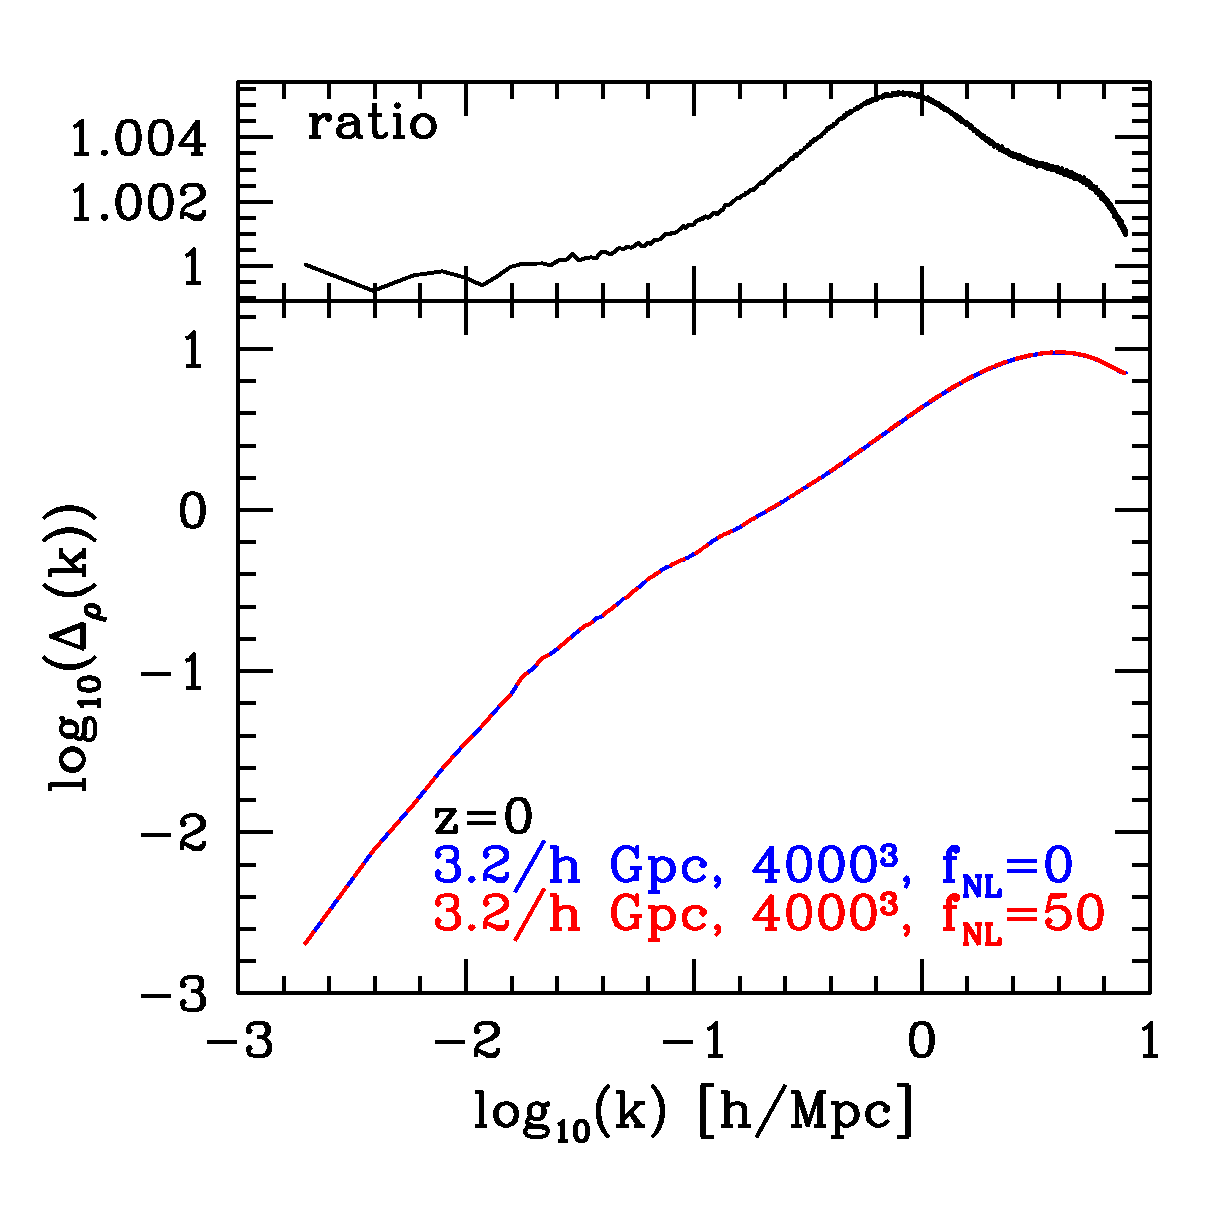
\includegraphics[width=3.2in]{graphs/dm_power_z0_fNL0_50.eps}
  \caption{ Dark matter power spectrum, measured at $z=0$ in a volume $3.2 h^{-1}\mbox{Gpc}$ per side,
  from $4000^3$ particles. The two curves represent two realizations of the same initial power spectrum, one of which used Gaussian statistics (blue) and the other the non-Gaussian initial condition generator. The to curves differ at the sub-per cent level, as seen in the top panel.   
    \label{fig:init}}
\end{center}
\end{figure}


\section{Other tools}

Particle ID, initial condition generator, projections, power spectrum code,  various expansions

\subsection{Extended range of the pp force}
\label{subsec:extendedpp}

One of the main source of error in the calculation of the force occurs when on the smallest scales of the fine grid.
The approximation by which particles in a neighbouring mesh grid can be placed at the centre of the cell
is less accurate, which cause a maximal scatter around the exact $1/r^2$ law.
A solution to minimize this error consists in extending the pp force calculation outside a single cell,
which inevitably reintroduces a $N^2$ number of operations. Our goal is to add the flexibility to have a code
that runs slower, but produces results with a higher precision. 

To allow this feature, we  have to choose how far outside a cell we want the exact pp force.  
Since the force kernels on both meshes are organized in terms of grids, the simplest way to implement this 
feature is to shut down the mesh kernels in a region of specified size, and allow the pp force to extend therein.
Concretely, these regions are constructed as cubic layers of fine mesh grids around a central cell; 
the freedom we have is to choose the number of such layers.
 
 To speed up the access to all particles within the domain of computation, we construct a thread safe linked list
 to be constructed and accessed in parallel by each core of the system, but this time with a head-of-chain that points to the first particle in the current fine mesh cell. We then loop over all fine grids, accessing the particles contained therein and inside each fine grid cells for which we killed the mesh kernels,
 we compute the separation and the force between each pairs and update their velocities simultaneously with Newton's third law. 
 To avoid double counting, we loop only over the fine mesh neighbours that produce non-redundant contributions. Namely, for a central cell located at 
 $(x_1, y_1, z_1)$, we only consider the neighbours $(x_2, y_2, z_2)$ that satisfy the following conditions:
 \begin{itemize}
 \item{$z_2 \ge z_1$ always}
 \item{if $z_2 = z_1$, then $y_2 \ge y_1$, otherwise we also allow $y_2 < y_1$} 
 \item{if $z_2 = z_1$ and $y_2 = y_1$, then we enforce $x_2 > x_1$}
 \end{itemize}
 The case where all three coordinates are equal is already calculated in the standard configuration of the code.
 
 To quantify the accuracy improvement versus computing time requirements, we performed the following test.
 We generate a set of initial conditions at a starting redshift of $z = 100$, with a box size equal to $ 200 h^{-1}\mbox{Mpc}$,
 and with $128^{3}$ particles. We evolve the particles to $z=0$ with different ranges for the pp calculation, and compare 
 the resulting power spectra. For the results to be meaningful, we also need to use the same random seed for the random number generator,
 such that the only difference between different runs is the range of the pp force.
 Fig. \ref{fig:power} shows the dimensionless power spectrum of the different runs, where we see a significant gains in resolution
 when extending  PM to P$^{3}$M first, and when adding successive layers of fine cell mesh where the pp force is extended.
We have not plotted the results for higher numbers of layers, as the improvement becomes milder there: the fine grid calculations
are more accurate as the distance increases. For this reason, it seems that a range of a few layers, between 3 and 6, suffices 
to reduce most of the undesired NGP scatter.

Extending the pp calculation comes at a price, since the number of operation scales as  $N^{2}$ in the sub-domain. 
This cost is best capture by the increase of real time required by a fixed number of dedicated  {\small CPU}s 
to evolved the particles to the final redshift. Table \ref{table:cpu_pp_ext} presents this usage.

\begin{figure}
  \begin{center}
  \epsfig{file=graphs/pp_ext.eps,width=0.49\textwidth,height=0.49\textwidth}
  \caption{ Dimensionless power spectrum for varying range of the exact pp force, compared to  {\small CAMB} \citep{Lewis:1999bs}.}
    \label{fig:power}
  \end{center}
\end{figure}


\begin{table}
\begin{center}
\caption{Scaling in {\small CPU} resources as a function of the range of the pp interaction.
$N_{layers}$ refers to the number of fine mesh layers around a given cell, inside of which the force calculation
is purely given by the pp contribution. }
\begin{tabular}{|l|c|c|}
\hline 
             Type         & time (h)   \\
                  \hline
PM                         & 1.77 \\
P$^{3}$M             & 2.09 \\
\hline
 $N_{layers}=1$ & 8.74 \\
 $N_{layers}=2$ & 11.47\\
 $N_{layers}=3$ & 14.30 \\
 $N_{layers}=4$ & 18.87\\
 $N_{layers}=5$ & 22.52\\
 $N_{layers}=6$ & 29.62\\
 $N_{layers}=7$ & 34.82\\
 $N_{layers}=8$ & 47.00\\
 

\hline \hline
\end{tabular}
\label{table:cpu_pp_ext}
\end{center}
\end{table}

Another way to quantify the improvement of the calculation is to look at the halo mass function for these different runs.
{\bf (To do...)}

%\subsection{Generalization of the dark energy equation of state}
%\label{subsec:runningomegal}
%
%The cosmic expansion is obtained from a third order Taylor expansion in the scale factor of Friedmann's equation,
%and has now the flexibility to accomodate a running equation of state of the form $\omega(a) = \omega_0 + a\omega_1$,
%which is the standard parameterization adopted by the Dark Energy Task Force \citep{2006astro.ph..9591A}.
%The code also currently supports expansion under a modified Chaplygin gas cosmology\cite{Chaplygin}. 
%{\bf Is this worth mentioning at all?}

%{}
 

\section{Conclusion}

The code is publicly available on github.com under {\tt cubep3m}, and extra documentation about the structure, 
compiling and running strategy is can be found at {\tt www.wiki.cita.utoronto.ca/mediawiki/index.php/CubePM}.

\section*{Acknowledgements}

%\input{Appendix}
\bibliographystyle{mn2e}
\bibliography{mybib3_new}{}
%\bibliographystyle{amsplain}

\bsp

\label{lastpage}


\end{document}
